\section{功能需求}
\subsection{CPU}

CPU的总体设计图如下图所示。

\thispagestyle{empty}
 % 流程图定义基本形状
\tikzstyle{startstop} = [rectangle, rounded corners, minimum width=3cm, minimum height=1cm,text centered, draw=black, fill=red!30]
\tikzstyle{io} = [trapezium, trapezium left angle=70, trapezium right angle=110, minimum width=3cm, minimum height=1cm, text centered, draw=black, fill=blue!30]
\tikzstyle{process} = [rectangle, minimum width=3cm, minimum height=1cm, text centered, draw=black, fill=orange!30]
\tikzstyle{decision} = [diamond, minimum width=3cm, minimum height=1cm, text centered, draw=black, fill=green!30]
\tikzstyle{arrow} = [thick,->,>=stealth]
 
\begin{center}
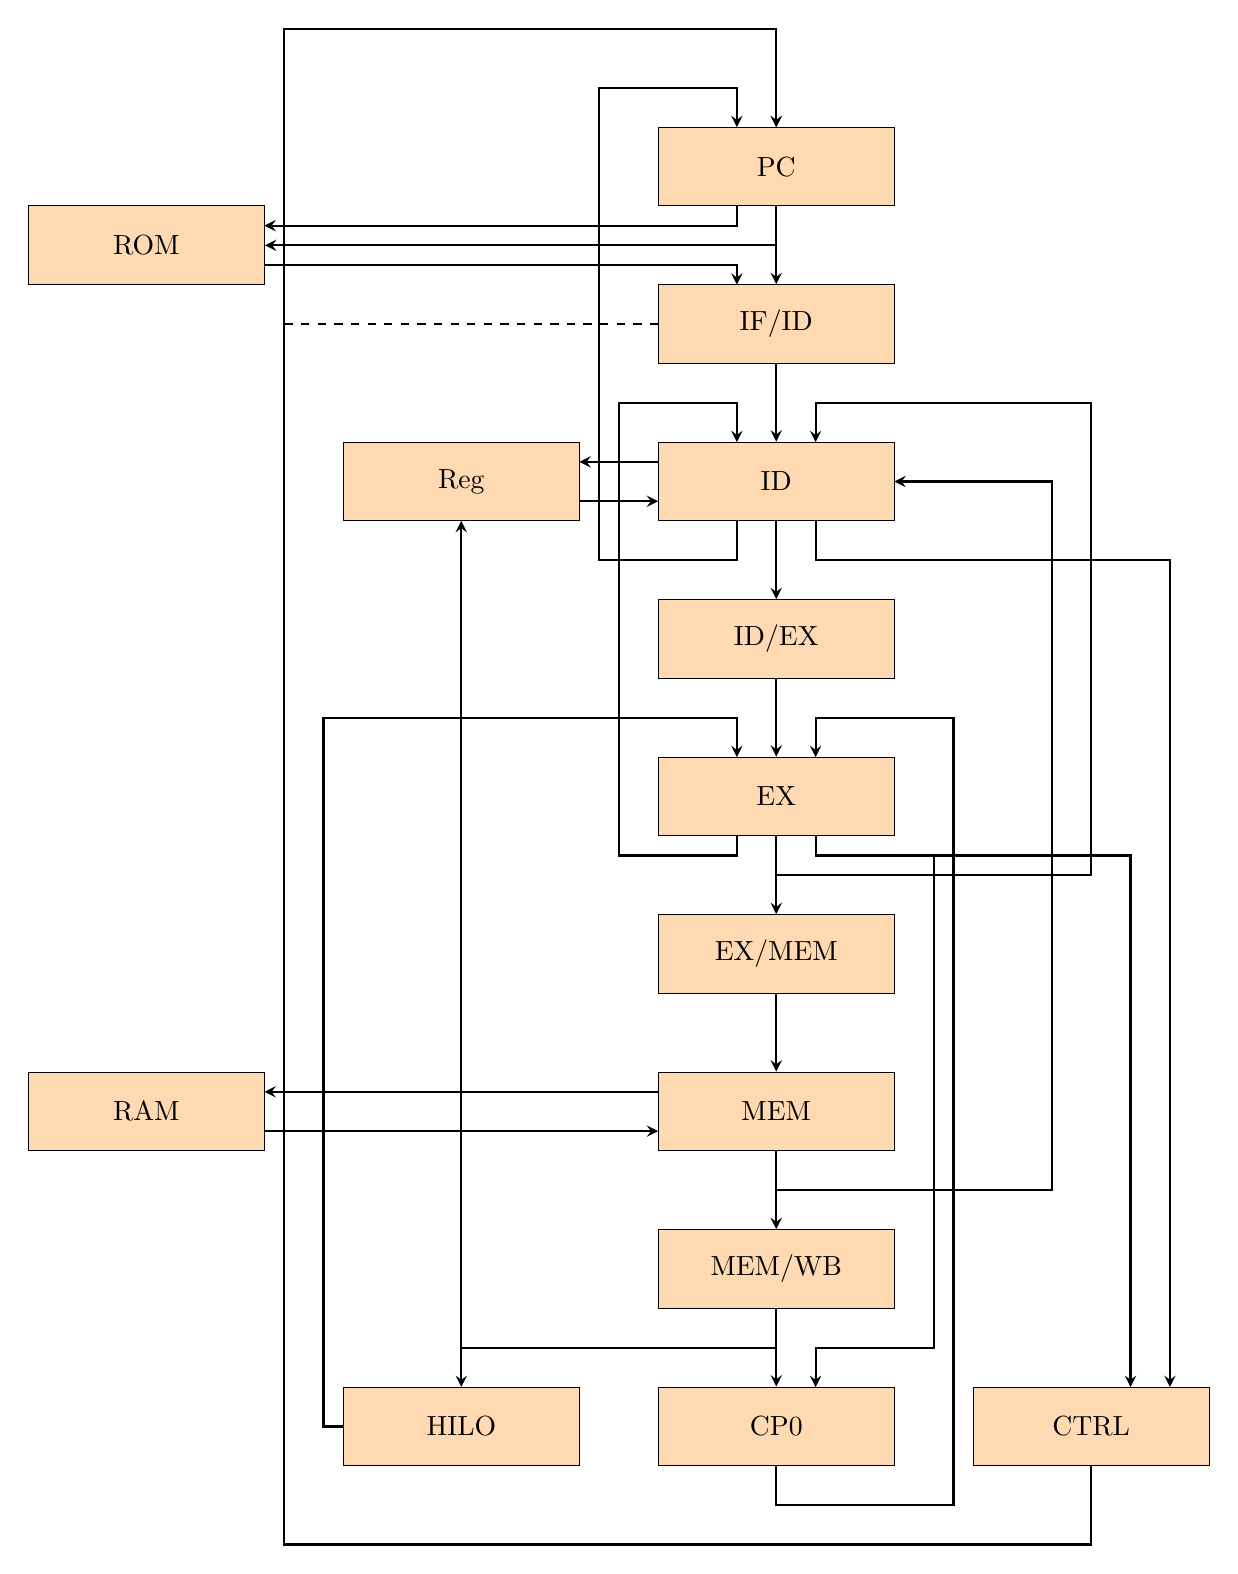
\begin{tikzpicture}[node distance=2cm]
 %定义流程图具体形状
\node (PC) [process] {PC};
\node (IFID) [process, below of=PC] {IF/ID};
\node (ROM) [process, left of=IFID, xshift=-6cm, yshift=1cm] {ROM};
\node (ID) [process, below of=IFID] {ID};
\node (Reg) [process, left of=ID, xshift=-2cm] {Reg};
\node (IDEX) [process, below of=ID] {ID/EX};
\node (EX) [process, below of=IDEX] {EX};
\node (EXMEM) [process, below of=EX] {EX/MEM};
\node (MEM) [process, below of=EXMEM] {MEM};
\node (RAM) [process, left of=MEM, xshift=-6cm] {RAM};
\node (MEMWB) [process, below of=MEM] {MEM/WB};
\node (CP0) [process, below of=MEMWB] {CP0};
\node (HILO) [process, left of=CP0, xshift=-2cm] {HILO};
\node (CTRL) [process, right of=CP0, xshift=2cm] {CTRL};
 
%连接具体形状
%PC
\draw [arrow](PC) -- (IFID);
\draw [arrow](PC) |- (ROM);
\draw [arrow](-0.5, -0.5) -- (-0.5, -0.75) -- (-6.5, -0.75);

%IFID
\draw [arrow](IFID) -- (ID);
\draw [arrow, dashed](-1.5, -2) -| (-6.25, 1.75) -| (0, 0.5);

%ROM
\draw [arrow](-6.5, -1.25) -- (-0.5, -1.25) -- (-0.5, -1.5);

%ID
\draw [arrow](-1.5, -3.75) -- (-2.5, -3.75);
\draw [arrow](ID) -- (IDEX);
\draw [arrow](-0.5, -4.5) |- (-2.25, -5) |- (-0.5, 1) -- (-0.5, 0.5);
\draw [arrow](0.5, -4.5) |- (5, -5) -- (5, -15.5);

%REG
\draw [arrow](-2.5, -4.25) -- (-1.5, -4.25);

%IDEX
\draw [arrow](IDEX) -- (EX);

%EX
\draw [arrow](EX) -- (EXMEM);
\draw [arrow](-0.5, -8.5) |- (-2, -8.75) |- (-0.5, -3) -- (-0.5, -3.5);
\draw [arrow](0, -9) -| (4, -3) -| (0.5, -3.5);
\draw [arrow](0.5, -8.5) |- (4.5, -8.75) -- (4.5, -15.5);
\draw [arrow](2, -8.75) |- (0.5, -15) -- (0.5, -15.5);

%EXMEM
\draw [arrow](EXMEM) -- (MEM);

%MEM
\draw [arrow](MEM) -- (MEMWB);
\draw [arrow](-1.5, -11.75) -- (-6.5, -11.75);
\draw [arrow](0, -13) -| (3.5, -4) -- (1.5, -4);

%RAM
\draw [arrow](-6.5, -12.25) -- (-1.5, -12.25);

%MEMWB
\draw [arrow](MEMWB) -- (CP0);
\draw [arrow](0, -15) -| (-4, -4.5);
\draw [arrow](-4, -15) -- (-4, -15.5);

%CP0
\draw [arrow](0, -16.5) |- (2.25, -17) |- (0.5, -7) -- (0.5, -7.5);

%HILO
\draw [arrow](-5.5, -16) -| (-5.75, -7) -| (-0.5, -7.5);

%CTRL
\draw [arrow](CTRL) |- (-6.25, -17.5) |- (0, 1.75) -- (0, 0.5);

\end{tikzpicture}
\end{center}

\subsubsection{ALU}
算术逻辑单元负责实现双输入的算术、逻辑和移位运算功能,其中包括乘法运算。

算术逻辑单元的输入端为两个32位整数和一个8位操作码,输出端为32位整数(乘法运算除外),并给出相应的标志位。

由于算术逻辑单元需要实现的运算种类较多,我们在此不做列举。

\subsubsection{乘法器}
乘法器负责实现乘法功能,输入为两个32位整数,输出为一个64位整数,分别存放在LO和HI两个32位寄存器中。

乘法运算采用Verilog语言提供的乘法运算符实现。我们没有将乘法器作为一个独立的元件来实现,而是在ALU中加入乘法的操作码,将乘法器并入算术逻辑单元实现。

考虑到乘法运算需要的时间比较长,如果乘法指令需要多周期完成,那么控制模块就必须暂停流水线,等待乘法指令完成后再让流水线恢复运作。为避免这种情况发生,可适当降低时钟频率,以使乘法运算可以在一个时钟周期内完成运算。

\subsubsection{寄存器堆}
寄存器堆负责实现通用寄存器的读写和在数据通路中的控制,在流水线译码阶段读取一个或两个通用寄存器的数据(组合逻辑电路),并在流水线写回阶段将结果写入通用寄存器(时序逻辑电路)。

32位MIPS架构需要实现32个32位通用寄存器,寄存器堆采用FPGA的逻辑单元来实现数据的存储,因此读写速度比内存快。

\subsubsection{CP0}
32位MIPS架构支持4个协处理器,本次实验需要实现CP0协处理器。CP0协处理器可以实现对TLB、MMU及异常处理的管理机制。

下表列出了CP0的寄存器及其功能,这里我们只给出必须实现的11个寄存器。

\begin{table}[H]
\centering
\begin{tabular}{lll}
\hline
编号&寄存器名称&寄存器功能\\
\hline
0&Index&用于TLBWI指令访问TLB入口的索引序号\\
2&EntryLo0&作为TLBWI及其他TLB指令接口,管理偶数页入口\\
3&EntryLo1&作为TLBWI及其他TLB指令接口,管理奇数页入口\\
9&BadVAddr&捕捉最近一次地址错误或TLB异常(重填、失效、修改)时的虚拟地址\\
10&Count&每隔一个时钟增加1,用作计数器,并可使能控制\\
11&EntryHi&TLB异常时,系统将虚拟地址部分写入EntryHi寄存器中用于TLB匹配信息\\
12&Compare&保持一定值,当Count值与Compare相等时,SI$\_$TimerInt引脚变高电平直到有数\\
&&值写入Compare,用于定时中断\\
13&Status&表示处理器的操作模式、中断使能及诊断状态\\
15&Cause&记录最近一次异常的原因,控制软件中断请求以及中断处理派分的向量\\
16&EPC&存储异常处理之后程序恢复执行的地址\\
18&EBase&识别多处理器系统中不同的处理器异常向量的基地址\\
\hline
\end{tabular}
\end{table}

\begin{enumerate}[(1)]
\item Index寄存器
Index寄存器是一个32位读/写寄存器,可用于TLBP、TLBR和TLBWI指令访问TLB入口的索引序号。

Index区域的大小根据具体实现方式随TLB的入口个数而定。对于基于TLB的内存管理单元MMU来说,该区域的最小值为$\lceil log_{2}(TLBEntries)\rceil$。

如果一个写入Index寄存器的值大于等于TLB入口数,则该处理器的操作是未定义的。

该寄存器仅对TLB有效。

\begin{table}[H]
\centering
\begin{tabular}{ccccccccccccc}
31&30&&&&&&6&5&&&&0\\
\hline
\multicolumn{1}{|c|}{P}&
\multicolumn{7}{c|}{0}&
\multicolumn{5}{c|}{Index}\\
\hline
\end{tabular}
\end{table}

\begin{table}[H]
\centering
\begin{tabular}{|c|c|c|c|c|}
\hline
\multicolumn{2}{|c|}{区域}&
\multirow{2}{*}{描述}&
\multirow{2}{*}{读/写}&
\multirow{2}{*}{重置状态}\\
\cline{1-2}
名称&比特&&&\\
\hline
\multirow{2}{*}{P}&
\multirow{2}{*}{31}&
\multicolumn{1}{l|}{检测故障。当先前的TLBProbe(TLBP)指令没有在TLB中寻}&
\multirow{2}{*}{R/W}&
\multirow{2}{*}{未定义}\\
&&
\multicolumn{1}{l|}{得匹配时,硬件会将其置为1。}&
&\\
\hline
0&30:6&
\multicolumn{1}{l|}{必须写为0;读取时返回0.}&
0&0\\
\hline
\multirow{3}{*}{Index}&
\multirow{3}{*}{5:0}&
\multicolumn{1}{l|}{TLB入口的索引值,收到TLBRead和TLBWrite指令影响。}&
\multirow{3}{*}{R/W}&
\multirow{3}{*}{未定义}\\
&&
\multicolumn{1}{l|}{对于16或32个入口的TLB,如果索引指向一个不存在的入口,}&
&\\
&&
\multicolumn{1}{l|}{则该行为是未定义的。}&
&\\
\hline
\end{tabular}
\end{table}

\item EntryLo1/EntryLo0寄存器
这对EntryLo寄存器的作用等同于TLB、TLBR、TLBWI和TLBWR指令间的接口。对基于TLB的MMU而言,EntryLo0管理偶数页的入口,EntryLo1管理奇数页的入口。如果出现了地址错误,TLB失效,TLB修改或是TLB重填异常的行为,那么EntryLo0和EntryLo1寄存器的内容将会成为未定义的。只有当基于TLB的存储管理单元存在时,这些寄存器才有效。

\begin{table}[H]
\centering
\begin{tabular}{cccccccccccccccccc}
31&30&29&&26&25&&&&&&6&5&&3&2&1&0\\
\hline
\multicolumn{2}{|c|}{R}&
\multicolumn{3}{c|}{O}&
\multicolumn{7}{c|}{PFN}&
\multicolumn{3}{c|}{C}&
\multicolumn{1}{c|}{D}&
\multicolumn{1}{c|}{V}&
\multicolumn{1}{c|}{G}\\
\hline
\end{tabular}
\end{table}

\begin{table}[H]
\centering
\begin{tabular}{|c|c|c|c|c|}
\hline
\multicolumn{2}{|c|}{区域}&
\multirow{2}{*}{描述}&
\multirow{2}{*}{读/写}&
\multirow{2}{*}{重置状态}\\
\cline{1-2}
名称&比特&&&\\
\hline
R&31:30&
\multicolumn{1}{l|}{保留区域。写入时应被忽略;读取时返回0.}&
R&0\\
\hline
\multirow{3}{*}{O}&
\multirow{3}{*}{29:26}&
\multicolumn{1}{l|}{在一般情况下,这4个位为PFN的一部分。但由}&
\multirow{3}{*}{R}&
\multirow{3}{*}{0}\\
&&
\multicolumn{1}{l|}{于24k仅支持32位的物理地址,PFN仅有20位}&
&\\
&&
\multicolumn{1}{l|}{的位宽,所以,该寄存器的29:26位强制写入0.}&
&\\
\hline
\multirow{2}{*}{PFN}&
\multirow{2}{*}{25:6}&
\multicolumn{1}{l|}{页帧号:有助于物理地址高位的定义。PFN区域}&
\multirow{2}{*}{R/W}&
\multirow{2}{*}{未定义}\\
&&
\multicolumn{1}{l|}{对应了物理地址的31~12位。}&
&\\
\hline
C&5:3&
\multicolumn{1}{l|}{页面一致性属性。}&
R/W&未定义\\
\hline
\multirow{3}{*}{D}&
\multirow{3}{*}{2}&
\multicolumn{1}{l|}{已使用或写使能位:表示了该页面已经被写入,并且}&
\multirow{3}{*}{R/W}&
\multirow{3}{*}{未定义}\\
&&
\multicolumn{1}{l|}{/或者是可写入的。如果D=1,则允许写入该页;如果}&
&\\
&&
\multicolumn{1}{l|}{D=0,则不允许写入该页,否则会引起TLB修改异常。}&
&\\
\hline
\multirow{4}{*}{V}&
\multirow{4}{*}{1}&
\multicolumn{1}{l|}{有效位:指明当前TLB入口是否有效,即虚拟页面映}&
\multirow{4}{*}{R/W}&
\multirow{4}{*}{未定义}\\
&&
\multicolumn{1}{l|}{射是否有效。如果该位为1,那么允许进入该页;如}&
&\\
&&
\multicolumn{1}{l|}{果V=1,则允许访问该页;如果V=0,访问该页会引}&
&\\
&&
\multicolumn{1}{l|}{起TLB无效异常。}&
&\\
\hline
\multirow{5}{*}{G}&
\multirow{5}{*}{0}&
\multicolumn{1}{l|}{全局位:在对TLB入口进行写操作时,EntryLo0和}&
\multirow{5}{*}{R/W}&
\multirow{5}{*}{未定义}\\
&&
\multicolumn{1}{l|}{EntryLo1寄存器中的G位与运算的结果作为TLB入}&
&\\
&&
\multicolumn{1}{l|}{口的G位。如果TLB入口的G位时1,ASID比较将在}&
&\\
&&
\multicolumn{1}{l|}{TLB匹配中被忽略掉。在对TLB入口进行读操作时,}&
&\\
&&
\multicolumn{1}{l|}{EntryLo0和EntryLo1的G位都反映了TLB的G位的状态。}&
&\\
\hline
\end{tabular}
\end{table}

\begin{table}[H]
\centering
\begin{tabular}{|c|l|}
\hline
C[5:3]值&
\multicolumn{1}{c|}{缓存一致性属性}\\
\hline
0&可缓存、非一致性、写通、无写分配\\
\hline
1&保留\\
\hline
2&不可缓存\\
\hline
3&缓存可、非一致性、写回、写分配\\
\hline
4,5,6&保留\\
\hline
7&无缓存加速\\
\hline
\end{tabular}
\end{table}

\item EntryHi寄存器
EntryHi寄存器包含了用于TLB读、写和访问操作的虚拟地址匹配信息。当TLB异常(TLB Refill,TLB Invalid或TLB Modified)发生时,系统将虚拟地址的[31:13]位写入EntryHi寄存器的VPN2区域。TLBR指令将选中的TLB入口相应的区域写入EntryHi寄存器。软件(通常是操作系统)将当前地址空间标识符写入ASID区域,该区域在TLB比较过程中用于确定TLB是否可以匹配。

由于ASID区域被TLBR指令重填覆盖了,软件必须保存和重新存储有关TLBR使用的ASID的值。这在发生TLB失效和TLB修改异常时,以及在其它存储管理软件中尤为重要。

在发生了地址错误的异常后,EntryHi寄存器的VPN2区域将成为未定义的,并且该区域可能在发生地址错误异常的过程中被硬件修改。EntryHi寄存器的软件写操作(通过MTC0)不会导致BadVAddr和Context寄存器中的地址相关区域发生隐式的写入(implicit write)。

\begin{table}[H]
\centering
\begin{tabular}{ccccccccccccccccc}
31&&&&&&&&13&12&&8&7&&&&0\\
\hline
\multicolumn{9}{|c|}{VPN2}&
\multicolumn{3}{c|}{0}&
\multicolumn{5}{c|}{ASID}\\
\hline
\end{tabular}
\end{table}

\begin{table}[H]
\centering
\begin{tabular}{|c|c|c|c|c|}
\hline
\multicolumn{2}{|c|}{区域}&
\multirow{2}{*}{描述}&
\multirow{2}{*}{读/写}&
\multirow{2}{*}{重置状态}\\
\cline{1-2}
名称&比特&&&\\
\hline
\multirow{3}{*}{VPN2}&
\multirow{3}{*}{31..13}&
\multicolumn{1}{l|}{虚地址(虚拟页面数目的一半)的$VA_{31..13}$。在TLB异常}&
\multirow{3}{*}{R/W}&
\multirow{3}{*}{未定义}\\
&&
\multicolumn{1}{l|}{或TLB进行读取时,该区域被硬件写入;在TLB写之前,}&
&\\
&&
\multicolumn{1}{l|}{该区域被软件写入。}&&\\
\hline
0&12..8&
\multicolumn{1}{l|}{必须写为0;在读取时返回0.}&
0&0\\
\hline
\multirow{3}{*}{ASID}&
\multirow{3}{*}{7..0}&
\multicolumn{1}{l|}{地址空间标识符。在TLB读取时,该区域由硬件写入;通过}&
\multirow{3}{*}{R/W}&
\multirow{3}{*}{未定义}\\
&&\multicolumn{1}{l|}{软件写该区域,可以为TLB写操作建立当前的ASID值,这}&&\\
&&\multicolumn{1}{l|}{样可以避免对TLB的访问匹配所有TLB入口的ASID值。}&&\\
\hline
\end{tabular}
\end{table}

该寄存器仅对TLB有效。

\item Status寄存器
Status寄存器是一个读/写寄存器,可以表示处理器的操作模式、中断使能以及诊断状态。该寄存器的区域联合作用,可以创建处理器的工作模式。

中断使能:当一下所有条件成立时启用中断:

\quad Status[0]:IE = 1

\quad Status[0]:EXL = 0

\quad Status[0]:ERL = 0

\quad 额外的:Debug[0]:DM = 0

当这些条件都符合时,设置IM(Status[16:9])位和IE位可以使能中断。

EXL与ERL任一位置1都可使系统进入Kernel模式,否则为User模式。

\item Cause寄存器
Cause寄存器主要记录最近一次异常的原因,也控制软件中断请求以及中断处理派分的向量。除了IP1..0、DC、IV和WP区域,Cause寄存器中其它的所有区域都是只读的。第二版架构在外部中断控制器(EIC)的中断模式下,增加了可选项。在这个模式下,IP7..2表示请求中断优先级(RIPL)。

Cause[6:2]表示ExcCode,即异常号。

\item Ebase寄存器
EBase寄存器是一个读/写寄存器,包含了在StatusBEV为0时所使用的异常向量的基地址及一个只读CPU号,该CPU号可以被软件用来区分多处理器系统中不同的处理器。

EBase寄存器使软件能在多处理器系统中识别特定的处理器,并允许每个处理器的异常向量可以不同,特别是对由多种处理器组成的系统。当StatusBEV为0时,EBase寄存器的位31:12由0构成,形成异常向量的基地址。当StatusBEV为1时,或在任何EJTAG调试异常的情况下,异常向量的基地址由固定的缺省值确定。

EBase寄存器的位31:30固定为2\#10,从而强制异常基地址在kseg0或kseg1的无映射的虚拟地址段中。在缓存错误异常中,异常基地址的位29将被强制置为1,从而使异常处理器从无缓存的kseg1段开始执行。如果需要改变异常基地址寄存器的值,则操作必须在StatusBEV为1的情况下进行。如果在StatusBEV为0时,在异常基地址区域写入了一个不同的值,处理器的操作将成为未定义的。

将位31:12与异常基地址区域相结合,可允许将异常向量的基地址置于任何4KB字节大小的页面的边界上。

\end{enumerate}

\begin{table}
\centering
\begin{tabular}{cccccccccccccccccc}
31&30&29&&&&&&&&12&11&10&9&&&&0\\
\hline
\multicolumn{1}{|c|}{1}&
\multicolumn{1}{c|}{0}&
\multicolumn{8}{c|}{Exception Base}&
\multicolumn{2}{c|}{0}&
\multicolumn{6}{c|}{CPUNum}\\
\hline
\end{tabular}
\end{table}

\begin{table}[H]
\centering
\begin{tabular}{|c|c|c|c|c|}
\hline
\multicolumn{2}{|c|}{区域}&
\multirow{2}{*}{描述}&
\multirow{2}{*}{读/写}&
\multirow{2}{*}{重置状态}\\
\cline{1-2}
名称&比特&&&\\
\hline
1&31&
\multicolumn{1}{l|}{在写入时,该位被忽略;在读取时,返回0.}&
R&1\\
\hline
\multirow{2}{*}{Exception}&
\multirow{2}{*}{29:12}&
\multicolumn{1}{l|}{与位31:30结合,该区域在$Status_{SEV}$为0时,指定了}&
\multirow{2}{*}{R/W}&
\multirow{2}{*}{0}\\
&&
\multicolumn{1}{l|}{异常的基地址。}&
&\\
\hline
\multirow{4}{*}{CPUNum}&
\multirow{4}{*}{9:0}&
\multicolumn{1}{l|}{该区域包含了一个标识符,它对多处理器系统的每个}&
\multirow{4}{*}{R}&
\multirow{4}{*}{外部设置}\\
&&
\multicolumn{1}{l|}{CPU都是唯一的。软件可以用此来判断它运行的位置。}&
&\\
&&
\multicolumn{1}{l|}{这个区域的值由连接到内核的$SI\_CPUNum[9:0]$静态}&
&\\
&&
\multicolumn{1}{l|}{输入管脚设置。}&
&\\
\hline
\multirow{2}{*}{0}&
30,&
\multicolumn{1}{l|}{必须写为0;在读取时返回0.}&
\multirow{2}{*}{0}&
\multirow{2}{*}{0}\\
&11:10&&&\\
\hline
\end{tabular}
\end{table}

通过调用MFC0,MTC0指令,CP0提供了统一的对外接口以完成对寄存器组的访问。\\\\
实现步骤:

\begin{enumerate}[(1)]
\item 选择要实现的CP0寄存器,可考虑推荐实现的寄存器或自行决定额外寄存器实现。

\item 按照CP0寄存器的功能分别在CPU的不同模块完成各寄存器的赋值。

\begin{enumerate}[(a)]
\item 在译码、运算及访存阶段发生地址错误时将错误地址赋值给BadVAddr

\item 异常处理开始时,若为TLB异常,则将错误地址高20位赋值给EntryHi高20位

\item 异常处理开始时,将Status[1]赋值为1;在执行ERET指令时将Status[1]赋值为0

\item 异常处理开始时,将Cause[6:2]赋值为异常号

\item 异常处理开始时,将EPC赋值为Victim指令地址

\item 每个周期,Count加1

\item 其他写操作由软件完成 
\end{enumerate}

\item 实现MFC0,MTC0指令访问CP0寄存器的功能。

\item 通过各寄存器值控制相应功能。

\end{enumerate}


\subsubsection{异常中断处理}
本次实验要求实现精确异常处理,即确定异常发生的位置,确保该指令前的指令全部执行完毕,并将该指令后的指令从流水线上擦除。

以下是一些可能用到的中断和异常的情况。

\begin{table}[H]
\centering
\begin{tabular}{lll}
\hline
异常号&异常名&描述\\
\hline
0&Interrupt&外部中断、异步发生,由硬件引起\\
1&TLB Modified&内存修改异常,发生在Memory阶段\\
2&TLBL&读未在TLB中映射的内存地址触发的异常\\
3&TLBS&写未在TLB中映射的内存地址触发的异常\\
4&ADEL&读访问一个非对齐地址触发的异常\\
5&ADES&读访问一个非对齐地址触发的异常\\
8&SYSCALL&系统调用\\
10&RI&执行未定义指令异常\\
11&Co-Processor Unavailable&试图访问不存在的协处理器异常\\
23&Watch&Watch寄存器监控异常\\
\hline
\end{tabular}
\end{table}

下表列出可能用到的中断号。

\begin{table}[H]
\centering
\begin{tabular}{ll}
\hline
中断号&设备\\
\hline
0&系统计时器\\
1&键盘\\
3&通讯端口COM2\\
4&通讯端口COM1\\
\hline
\end{tabular}
\end{table}

中断/异常处理的一般流程如下:

\begin{enumerate}[(1)]
\item 保存中断信息,主要是EPC,BadVaddr,Status,Cause等寄存器的信息

\qquad EPC:存储异常处理之后程序恢复执行的地址。对于一般异常,当前发生错误的指令地址即为EPC应当保存的地址;而对于硬件中断,由于是异步产生则可以任意设定一条并未执行完成的指令地址保存,但在进入下一步处理之前,该指令前的指令都应当被执行完。

\qquad BadVAddr:捕捉最近一次地址错误或TLB异常(重填、失效、修改)时的虚拟地址。

\qquad Status:将EXL位置为1,进入kernel模式进行中断处理。

\qquad Cause:记录下异常号。

\qquad EntryHi:TLB异常时,记录下BadVAddr的部分高位。

\item 根据Cause中的异常号跳转到相应的异常处理函数入口

\item 中断处理

\item 通过调用ERET指令恢复现场,返回EPC所存地址执行并且将Status中的EXL重置为0表示进入user模式。

\end{enumerate}

\quad \\
实现步骤:

\begin{enumerate}[(1)]
\item 在可能发生异常的位置实现对异常的记录。

\begin{enumerate}[(a)]
\item 访存时可能发生ADEL,ADES,TLBM,TLBL,TLBS,Watch异常

\item 译码后可能发生RI,SYSCALL,Co-ProcessorU异常
\end{enumerate}
\item 实现对中断的记录。

\begin{enumerate}[(a)]
\item 硬件产生中断时将信息写入CP0寄存器
\end{enumerate}

\item 根据异常记录信息判断是否产生异常。

\item 进入异常处理流程。

\end{enumerate}

\subsubsection{MMU}
内存管理单元负责实现虚拟地址转换到物理地址,再访问相应元件读取或写入数据的全过程,并实现内核态与用户态的区分。同时MMU还需要集成TLB模块,并实现相应的TLB异常处理。

\paragraph{物理地址划分}

\quad

\quad

\begin{table}[H]
\centering
\begin{tabular}{cll}
\hline
物理地址范围&设备&说明\\
\hline
$\left[ 0x00000000, 0x007FFFFF\right] $&RAM&共8MB\\
$\left[ 0x1FC00000, 0x1FC00FFF\right] $&引导ROM&共4KB\\
$\left[ 0x1E000000, 0x1EFFFFFF\right] $&flash&地址空间共16MB,但对于32位字,只有低16位有效\\
$\left[ 0x1A000000, 0x1A096000\right] $&VGA&\\
0x1FD003F8&串口数据&\\
0x1FD003FC&串口状态&\\
0x1FD00400&数码管&\\
0x0F000000&键盘码&\\
\hline
\end{tabular}
\end{table}

\paragraph{虚拟地址划分}

\quad

\quad

\begin{table}[H]
\centering
\begin{tabular}{clllc}
\hline
虚拟地址范围&名称&权限&MMU&物理地址范围\\
\hline
$\left[ 0x00000000, 0x7FFFFFFF\right] $&kuseg&内核/用户&是&-\\
$\left[ 0x80000000, 0x9FFFFFFF\right] $&kseg0&内核&否&$\left[ 0x00000000, 0x1FFFFFFF\right] $\\
$\left[ 0xA0000000, 0xBFFFFFFF\right] $&kseg1&内核&否&$\left[ 0x00000000, 0x1FFFFFFF\right] $\\
$\left[ 0xC0000000, 0xFFFFFFFF\right] $&kseg2&内核&是&-\\
\hline
\end{tabular}
\end{table}

\paragraph{TLB}

\quad

\quad

虚拟地址到物理地址的转换是通过查找页表来实现的,为了加速查询过程,CPU对页表进行缓存。如果虚拟地址在页表中没有找到相应的映射,将产生缺页异常,由操作系统将对应的页表项加入缓存,并继续进行访问操作。

本实验中硬件需要实现一组寄存器来存储页表的缓存,支持TLBWI语句,并和CP0协处理器配合工作,页表的管理和异常处理等则由软件实现。

TLB共有16个表项,每个表项有64位长,每项可以存储两个物理页,因此总共可以存储32个页。

每次页表项更新时,页表信息被存放在如下寄存器中:目录为$INDEX\left[ 3:0 \right]$,对应的每个表项入口为\\
$\left\lbrace EntryHi\left[ 31:13 \right], EntryLo1\left[ 25:6 \right],EntryLo1\left[ 2:1 \right], EntryLo0\left[ 25:6 \right], EntryLo0\left[ 2:1 \right] \right\rbrace $

即高22位存储了虚拟地址高22位,后面分别跟着两组物理地址(奇偶)及其标志位(Valid,Global),匹配虚拟地址与标志后将实地址合并得到物理地址。
\subsection{Ucore}
\subsubsection{BIOS}
BIOS即为启动ucore所用的Bootloader程序,通常是放在Flash中。本实验中我们将在FPGA里建立一块ROM,将Bootloader放置在该ROM中,并且设置CPU的访问地址从该ROM开始,这样能避免由于Flash的读写不稳定而对BIOS造成的破坏,还能将ucore与BIOS独立出来。

BIOS启动时,Flash中的操作系统加载到内存中,然后跳转到操作系统的初始化代码,从而开始操作系统的工作。
\subsubsection{远程文件执行}
修改ucore,实现简单的远程文件执行功能,即通过串口从PC上获取ELF文件,并在本地执行。
\subsection{外设}
\subsubsection{串口}
串口的功能需求为实现与PC机的通信,通过计算机键盘输入数据,向计算机输出数据。

串口模块波特率固定在115200,数据位8位,停止位1位,奇校验。

地址1FD003F8表示数据(仅低8位有效),必须使用SW命令写入。

地址1FD003FC表示状态寄存器Status,Status\&1=1时可写,Status\&2=2时可读。

\subsubsection{VGA}
Device$\_$VGA模块是显示控制模块,接受CPU写入的ASCII码数据,并维护一个字符矩阵,以字符中断的形式通过VGA接口输出到显示器。

CPU需要从地址1FC03000读出数据,如果结果为‘1’表示可以写入,否则不能写入。可以写入时,向该地址写入ASCII数据即可。

显示模块包含两个子模块:控制模块DisplayControl以及VGA模块VGA640480。

屏幕分辨率640*480,VGA时钟为25MHz。

屏幕划分为若干个8*16的小方格,方格总数为80*30。

为了能够显示所有ASCII码字符,事先生成了ASCII码对应的8*16点阵,存储在一块片上ROM里,由VGA640480模块调用。

DisplayControl模块内使用一块片上Ram存储80*30个方格对应的ASCII码,并由VGA640480模块调用进行查询。此外,DisplayControl模块接收外部给出的写信号,对字符进行写入。

\subsubsection{ps/2键盘}
Device$\_$Keyboard模块位键盘控制模块。从地址0F000000读出数据,结果为0表示没有新数据,否则读到的就是键入的ASCII码。

PS/2键盘读到的是扫描码,为了方便软件,可以在硬件层面加入编码转换,CPU读到的直接就是ASCII码。
\subsection{数据通路}
本实验将实现基于标准32位MIPS指令集的子集的五级流水CPU,支持异常、中断、TLB等。

MIPS指令集的各条指令可以分解为取指(IF)、译码(ID)、执行(EX)、访存(MEM)和回写(WB)五个阶段,分别对应于本次实验需要实现的五个核心模块。模块内部采用组合逻辑电路实现,相邻模块之间的数据传输采用时序逻辑电路实现,每经过一个时钟周期,所有阶段分别将各自保存的结果交给下一个阶段,从而实现流水CPU。

此外,我们还需要实现寄存器堆模块(Regfile)、HILO模块(HILO)、协处理器模块(CP0)和控制模块(CTRL)。寄存器堆模块在译码阶段实现,便于指令在译码阶段访问寄存器并得到相应的数据。HILO模块和协处理器模块在回写阶段实现。控制模块则用于控制整个流水线的暂停、清除等动作,因此不将其归入流水线中的某一个阶段。

流水线虽然能提高指令执行效率,但由此带来的冲突是不可避免的。流水线冲突主要有结构冲突、数据冲突和控制冲突三种类型。
\begin{enumerate}
\item 结构冲突

指令在重叠执行过程中发生硬件资源冲突,在MIPS架构中主要是指取指阶段和访存阶段同时对存储器进行访问引起的冲突。解决方法是在设计数据通路时,采用资源重复设置的方法。如果指令和数据放在同一个存储器,可使用双端口存储器,一个端口存取数据,另一个端口取指令,这两个操作可以并行操作而不引起结构冲突。

\item 数据冲突

在同时重叠执行的几条指令中,一条指令依赖于前面指令执行结果,但是得不到执行结果造成的冲突。解决方法是在数据通路中加入流水线暂停和恢复机制,并引入数据前推技术,将执行结果提前送到其他模块,以供其他模块参考和使用。

\item 控制冲突

流水线中的分支指令或者其他需要改写PC的指令造成的冲突。解决方法是引入延时槽机制,这要求编译器在分支指令后插入空指令,对流水线的性能有一定的影响。

\end{enumerate}

本次实验需要实现的MIPS32指令集详见附录,基本数据通路图详见设计文档。
